\section{Challenges of the conventional analysis methods}
In this section, I will briefly introduce the conventional analysis methods used in the field, 2 fundamental challenges faced with the current method, and discuss the existing approaches to address these challenges and their limitations. 

Fundamentally, experimental results capture the interaction between the probe and the target; To distill the scientific essence presented in the results, complex analysis are usually required. In the case of microscopy measurements like STM, conventional methods like \ac{FT} are commonly used. %todo: add citations on examples of FT microscopy.
The \ac{FT} reveals characteristic wavelengths and provides insights to the underlying scientific theories of the specimen studied; This is particularly true in cases where the microscopy results contain near perfect periodic features, but when aperiodic signals are presented, the \ac{FT} is less ideal and suffers from loss of information. 

There are 2 specific challenges in QPI analysis with conventional \ac{FT} method we would like to focus on, the speckle problem, and the demixing problem. We will also establish their mathematical formulations, which will lead to the convolutional data model we present later. 

\subsection{The Speckle problem}
As introduced in the end of Ch5 and theorized explicitly in Equation \ref{eq.539}, when we take \ac{FT} of the grid map on multiple occurrence of defects, we get speckles on the \ac{FT-STS}; The problem is that the spatial distribution information of the defect location manifest as undesirable patterns in the \ac{FT} space, and makes the QPI pattern hard to interpret.

Therefore, to address the challenge of speckles is to disentangle the spatial information from the \ac{QPI} pattern, and this can be formulated mathematically as a deconvolution problem. 

\par \noindent Recall that we can write the modulation of \ac{LDOS} $\delta \rho$ from multiple defects as:
\begin{equation}
	\delta \rho(\mathbf{x}, \omega) = \sum_{j=1}^{N}c_j \cdot \delta \rho_0(\mathbf{x}-\mathbf{x_j},\omega),
\end{equation}
\noindent where $\delta \rho_0$ is the \ac{LDOS} modulation from individual defect located at at $\mathbf{x_j}$. We can further separate the spatial information by utilizing a Kronecker delta $\Delta(\mathbf{u})$, so that $\Delta(\mathbf{u})=1$ if $\mathbf{u} = 0$, and $\Delta(\mathbf{u})=0$ elsewhere: 
\begin{equation}
	\sum_{j=1}^{N}c_j \cdot \delta \rho_0(\mathbf{x}-\mathbf{x_j},\omega) = \sum_{\mathbf{u}} \delta \rho_0(\mathbf{x}-\mathbf{u},\omega)\cdot(\sum_{j=1}^{N} c_j \cdot \Delta(\mathbf{u-x_j})).
\end{equation}
\noindent We can then construct a convolution sum between the individual \ac{QPI} pattern and the spatial information by defining a defect location function $D(\mathbf{x}) \equiv \sum_{j=1}^{N} c_j \cdot \Delta(\mathbf{u-x_j})$, we have: 
\begin{equation}
	\delta \rho(\mathbf{x}, \omega) =  \sum_{\mathbf{u}} \delta \rho_0(\mathbf{x}-\mathbf{u},\omega)\cdot D(\mathbf{u}) = (\delta \rho_0 *D)(\mathbf{x}, \omega).
\end{equation}

We illustrate this convolution in Fig. \ref{fig:ch6_decon}; First, we use $\delta \rho_0$ simulated in Ch.5.2 as the \ac{QPI} pattern from an single defect, we then randomly generate a binary defect location map given a defect density, and use the convolution sum to construct an observation Y. To unify the language, we will refer the single defect \ac{QPI} pattern as a kernel, denoted as A; and the defect location map as an activation map, denoted as X. Therefore, our goal is that given $Y = A * X$, we want to reconstruct A and X. 

\begin{figure}
	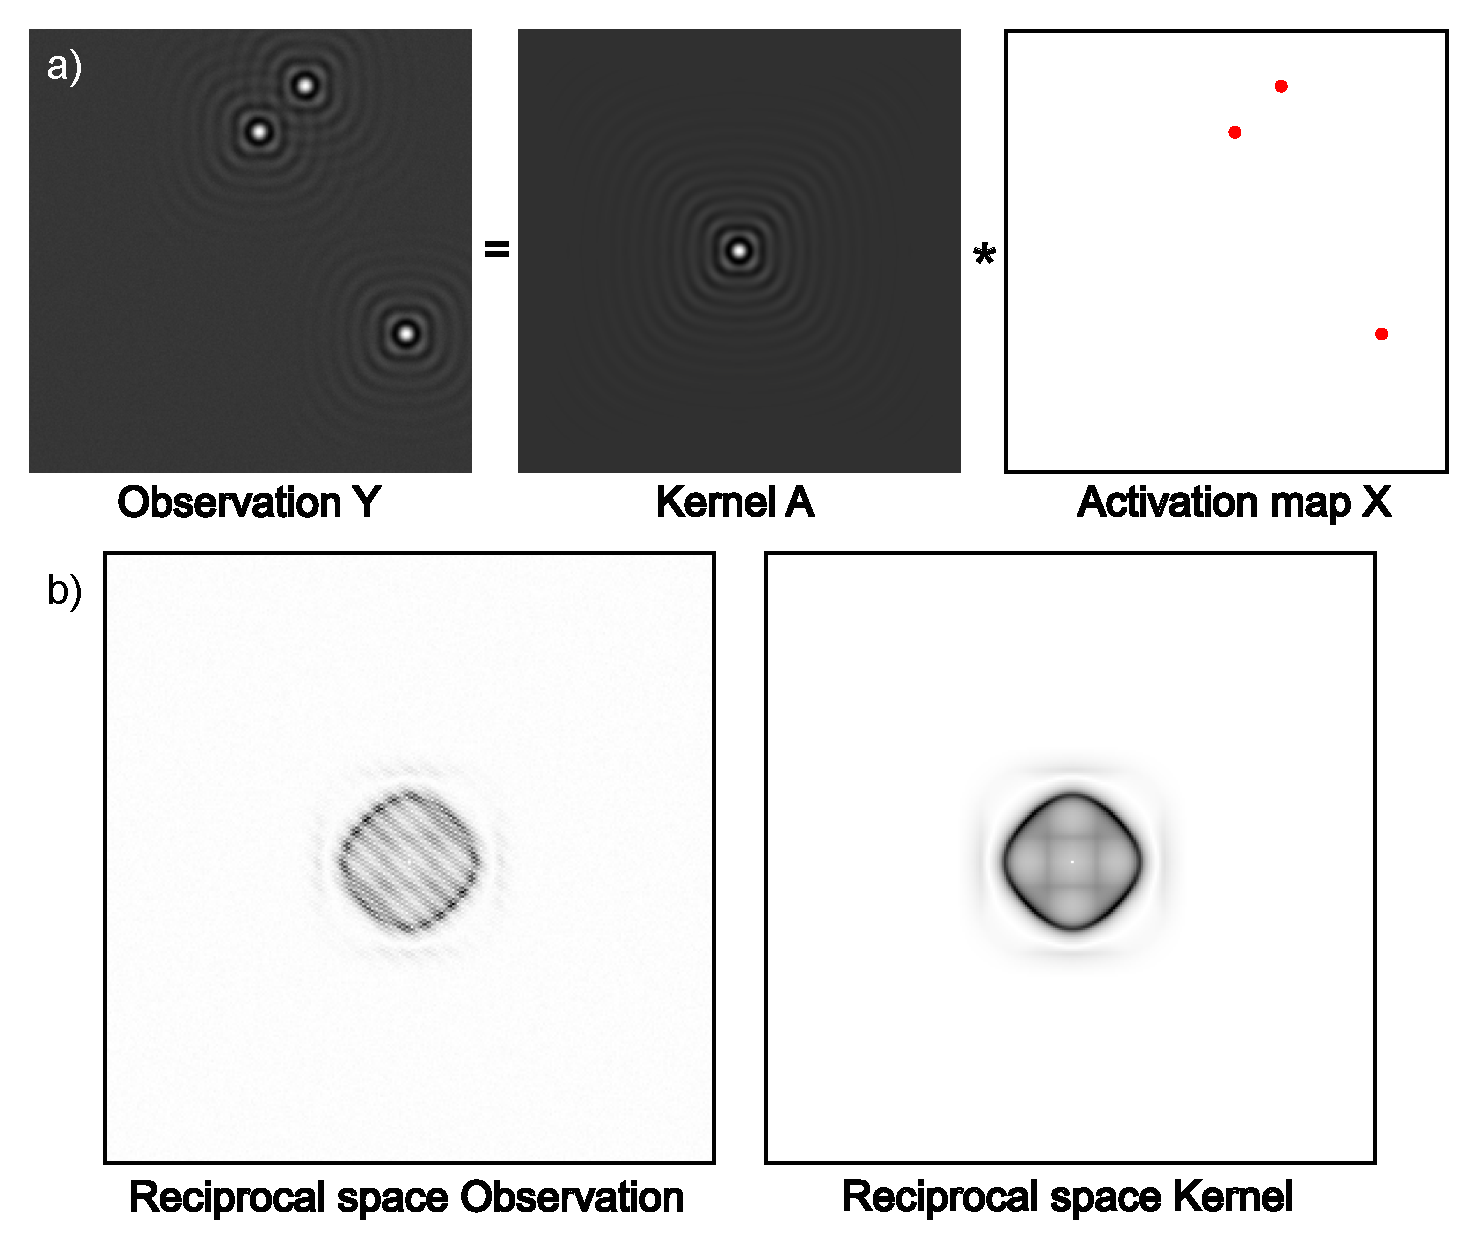
\includegraphics[width= \textwidth]{Ch6_deconvolution.pdf} 
	\centering
	\caption{}
	\label{fig:ch6_decon}
\end{figure}

\subsection{The Demixing problem}
%todo: how should I include the general motivation of demxing? or is it enough here? 
Materials normally exhibit multiple types of defects, and these defects can present different scattering features; Many QPI measurements have exploited the mechanisms of selectivity scattering channels across a wide variety of materials, such as the sign variation of the superconducting order parameter, the spin and orbital texture of topological bands, etc. However, there are only limited approaches to analyze and disentangle defect dependent scattering features. The most common approach is to acquire grid spectroscopy on isolated defects, or to crop around individual defect in larger grid maps if isolated defect is hard to find. One example is the Dirac semimetal ZrSiS, where the interference patterns around impurities located on the Zr and S sublattice sites scatter differently \cite{butler et al}; As shown in \ref{fig:ch6_ZrSiS}, conventional \ac{FT} display a mixture of the scattering features, which are disentangled through inspecting the \ac{FT} of cropped grid spectroscopy around individual defects. 

There are 2 primary shortcomings with this approach, one is due to small spatial range of the cropping, the resolution in q-space is very much limited, making it hard to resolve features with higher frequencies. Second is that the cropped area could still preserve features from other defect sources, this is particularly problematic when we have quasiparticles with longer lifetime; The long decaying tail could easily spread tens or hundreds of unit cells, making it hard to avoid when cropping. 

\begin{figure}
	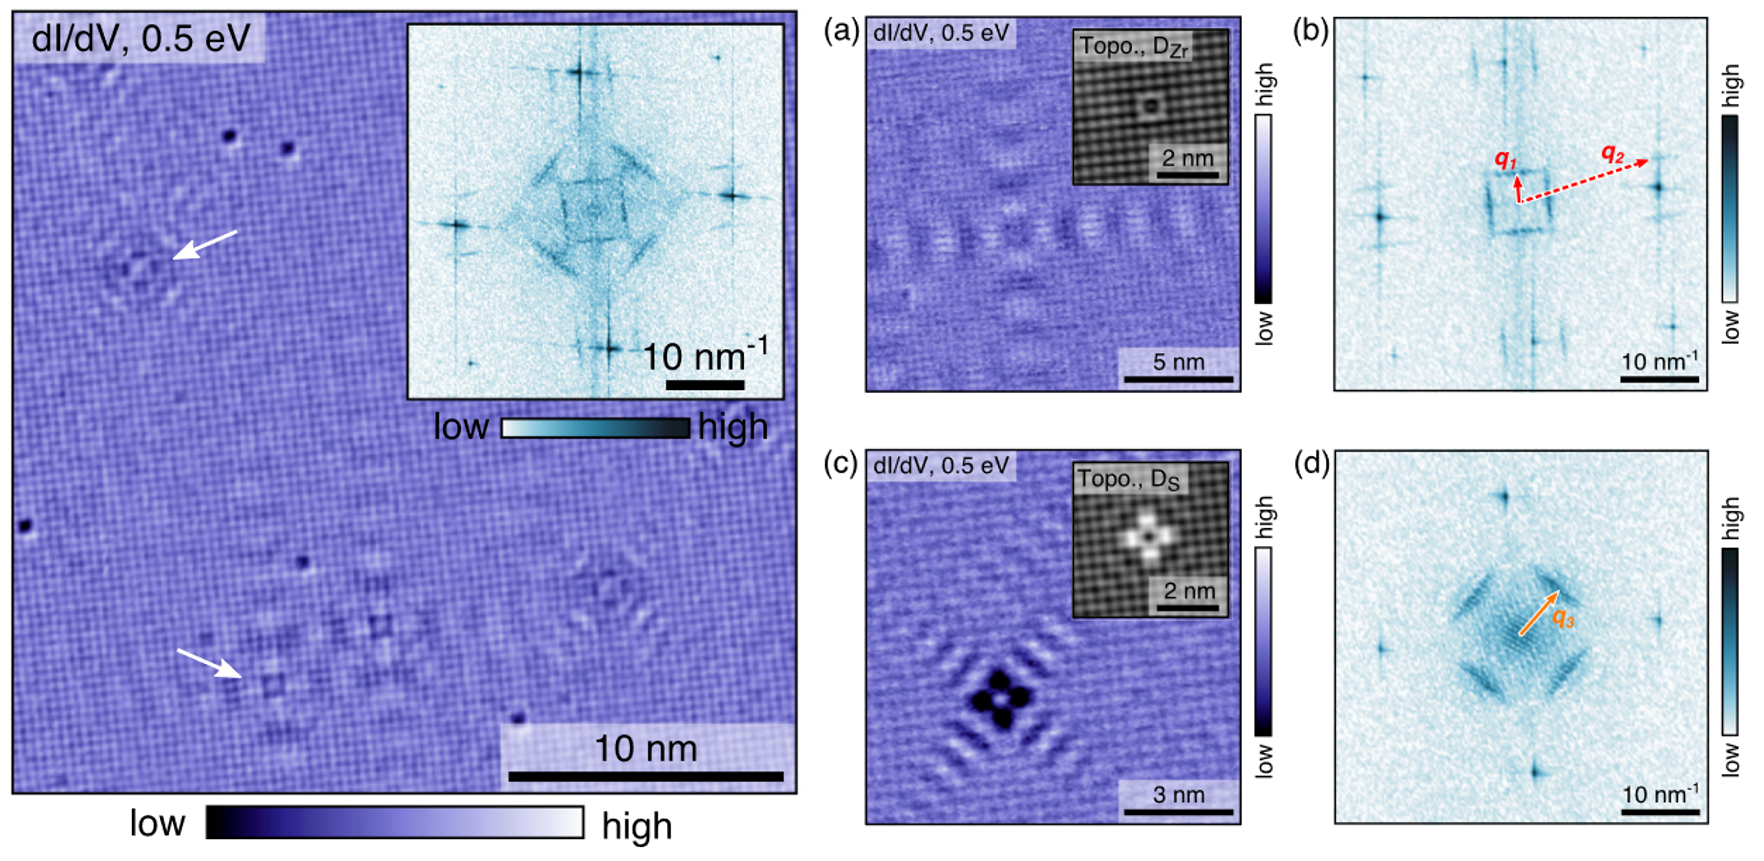
\includegraphics[width= \textwidth]{ZrSiS.png} 
	\centering
	\caption{}
	\label{fig:ch6_ZrSiS}
\end{figure}
%todo: add citations to corresponding literatures 

It is therefore preferred, if we can reconstruct the contribution of each individual type of defect from a big grid map that includes multiple types of defects; this is called the demixing problem.  

We now use our synthetic data to better illustrate the demixing problem. We simulate 2 \ac{QPI} patterns from 2 distinct defects with kernel choices A1 and A2 as shown in Fig. \ref{fig:ch6_demix} c) and d); We then define their activation maps X1 and X2 in d) and g). By summing up the convolutions between 2 kernels and their corresponding activation maps, we can obtain an observation Y in a). We express the above observation generation process as:

\begin{equation}
	Y = A1 * X1 + A2 * X2 + \beta, 
\end{equation}
where $\beta$ is the added noise determined by a pre-defined signal-to-noise ratio.

The demixing problem is the inverse of the observation generation process: given the observation 
Y, our goal is to reconstruct A1, A2, and their corresponding activation maps. This means that in reciprocal space, rather than working with entangled and less informative data like (b), we can recover disentangled QPI patterns from individual defect types, as shown in (e) and (h), which are also free from speckles. Lastly, we extend the above formulation with multiple types of different defects, then at arbitrary energy $\omega$, we have: 

\begin{equation}
	\label{eq:demixing}
	Y_{\omega} = \sum_d ( A_{d,{\omega}} * X_d) + \beta. 
\end{equation} 

\begin{figure}
	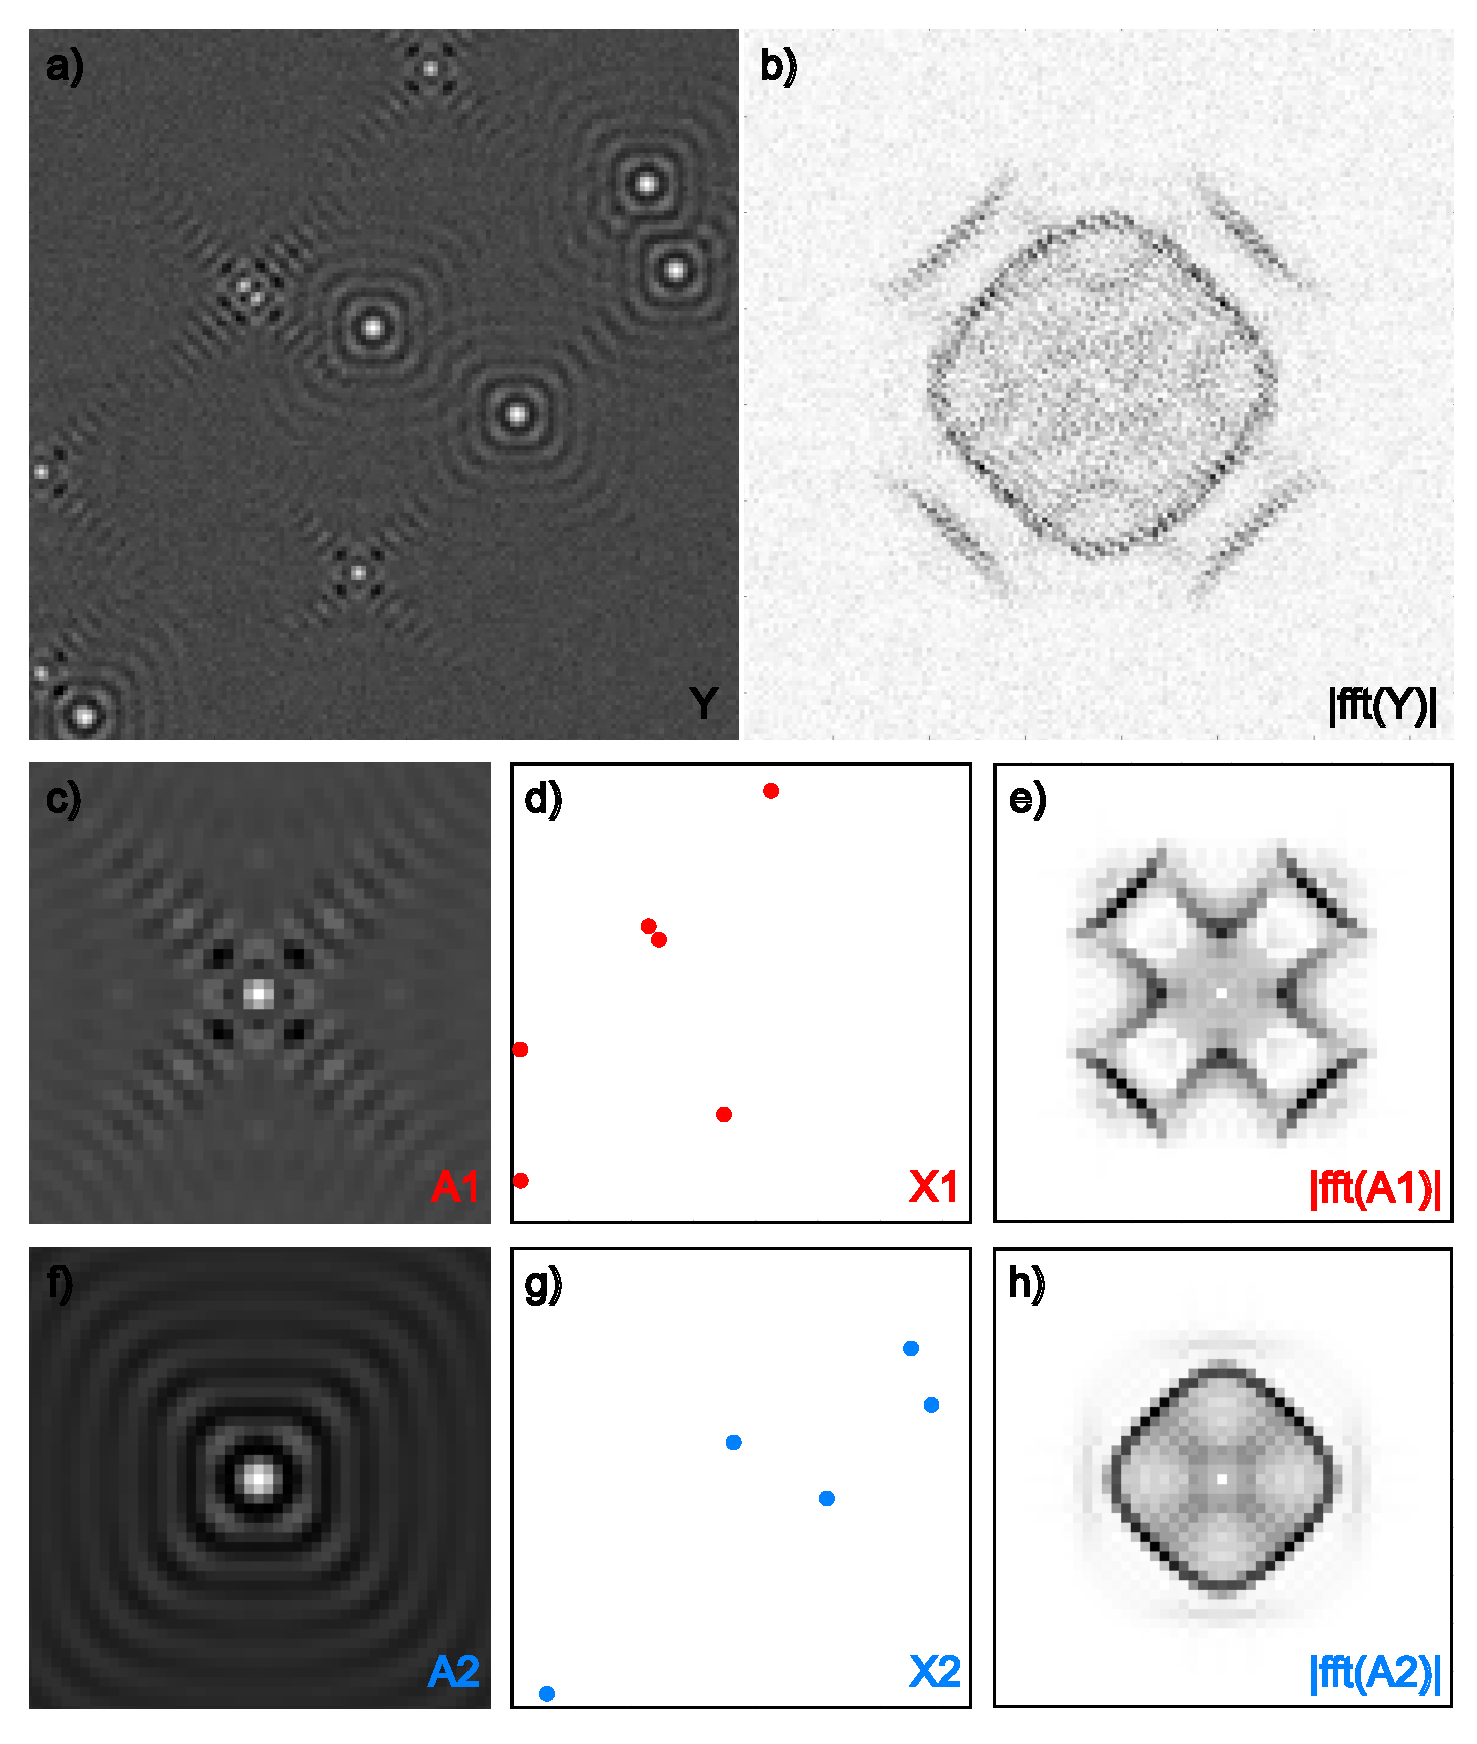
\includegraphics[width= \textwidth]{Ch6_demixing.pdf} 
	\centering
	\caption{}
	\label{fig:ch6_demix}
\end{figure}


